% Chapter Template

\chapter{State-of-the-art} % Main chapter title

\label{Chapter2} % Change X to a consecutive number; for referencing this chapter elsewhere, use \ref{ChapterX}

\lhead{Chapter 2. \emph{State-of-the-art}} % Change X to a consecutive number; this is for the header on each page - perhaps a shortened title

%----------------------------------------------------------------------------------------
%	SECTION 1
%----------------------------------------------------------------------------------------
\section{Introduction}
This chapter will review research literature in the field of machine learning and credit scoring. We 



%----------------------------------------------------------------------------------------
%	SECTION 2
%----------------------------------------------------------------------------------------
\section{Modelling Credit Risk SMEs}
How and why sme modelling is usually done completed in a financial institution



%----------------------------------------------------------------------------------------
%	SECTION 3
%----------------------------------------------------------------------------------------
\section{Macro Area Features affecting SME Credit Risk}
Details examples where features have been used to predict arrears

\cite{hackbarth_capital_2006} note that even though there has been a substantial amount of time  understanding and developing the credit risk literature, there not been much time spent researching how macroeconomic factors affect credit risk.  \cite{hackbarth_capital_2006} finds this strange based on anecdotal suggestions from institutions that economic business cycle is an important feature when calculating the probability of default of a customer. One example of this is during a recession we know consumers are less likely to spend money on discretionary goods or luxuries thus as a result businesses in a sector that offer these goods credit risk will most likely rise.

\cite{fama_term_1986} notes how over the counter derivatives broker-dealers measure risk using individual counter-parties details but also geographic data and performance indicators of other industry groups. The \cite{derivatives_policy_group_framework_1995} \footnote{The Derivatives Policy Group was made up of representatives of CS First Boston, Goldman Sachs, Morgan Stanley, Merrill Lynch, Salomon Brothers, and Lehman Brothers} also made recommendations that credit exposure was measured by geography and industry exposure when calculating credit risk.

Banks can also suffer from a risk known as the \textit{winners curse}. In banking this is a scenario where other banks credit risk models score a customer too risky to lend to. That party then arrives at "our bank" where "our model" scores them as a good or likely to repay customer and decide to lend to them. As a result "our bank" will take on an excessive amount of risk that where other banks expected loses \citep{duffie_credit_2012}. \cite{duffie_credit_2012} also discuss how banks can mitigate their risk to the winners curse by including metrics such as borrowing rates and credit risk concentration limits by area or location.

\citep{di_pietro_regional}

\textit{The analysis shows that, when the value of the aggregate shock shifts between different
	states (boom or recession), the shareholders’ default policy is characterized by a different
	default threshold for each state. \cite{hackbarth_capital_2006}}




\subsubsection{Location/Geospatial Data in Predictive Modelling}
This will include details on location metrics and there use in predictive modelling. I will also be including details on what electoral divisions/local authorities are.

\begin{comment}
The geography of the data  Provinces  Ireland is divided into four provinces: Leinster, Ulster, Munster and Connacht. Although at present they do not have any  administrative functions, they are relevant for a number of historical, cultural and sporting reasons. The borders of the  provinces coincide exactly with the boundaries of the administrative counties. Three of the nine counties in Ulster are  within the jurisdiction of the State.  NUTS boundaries  The Nomenclature of Territorial Units for Statistics (NUTS) were drawn up by Eurostat in order to define territorial  units for the production of regional statistics across the European Union. The NUTS classification has been used in EU  legislation since 1988, but it was only in 2003 that the EU Member States, the European Parliament and the  Commission established the NUTS regions within a legal framework.  The Irish NUTS 3 regions comprise the eight Regional Authorities established under the Local Government Act, 1991  (Regional Authorities) (Establishment) Order, 1993 which came into operation on January 1st 1994. The NUTS 2  regions, which were proposed by Government and agreed to by Eurostat in 1999, are groupings of the Regional  Authorities.  Administrative counties  In census reports the country is divided into 29 counties/administrative counties and the five Cities which represent the  local authority areas. Outside Dublin there are 26 administrative counties (North Tipperary and South Tipperary each  ranks as a separate county for administrative purposes) and four Cities, i.e. Cork, Limerick, Waterford and Galway. In  Dublin the four local authority areas are identified separately, i.e. Dublin City and the three administrative counties of  Dún Laoghaire-Rathdown, Fingal and South Dublin.  Electoral Divisions  There are 3,440 Electoral Divisions (EDs) which are the smallest legally defined administrative areas in the State. One  ED, St. Mary's, straddles the Louth-Meath county border, and is presented in two parts in the SAPS1 tables, with one  part in Louth and the other in Meath. There are 32 EDs with low population, which for reasons of confidentiality have  been amalgamated into neighbouring EDs giving a total of 3,409 EDs which appear in the SAPS tables.  Small Areas  Small Areas are areas of population comprising between 50 and 200 dwellings created by The National Institute of  Regional and Spatial Analysis(NIRSA) on behalf of the Ordnance Survey Ireland(OSi) in consultation with CSO. Small  Areas were designed as the lowest level of geography for the compilation of statistics in line with data protection and  generally comprise either complete or part of townlands or neighbourhoods. There is a constraint on Small Areas that  they must nest within Electoral Division boundaries.  Small areas were used as the basis for the Enumeration in Census 2011. Enumerators were assigned a number of  adjacent Small Areas constituting around 400 dwelling in which they had to visit every dwelling and deliver and collect  a completed census form and record the dwelling status of unoccupied dwellings.  The small area boundaries have been amended in line with population data from Census 2011  2007 Constituency boundaries  For the purpose of elections to Dáil Éireann the country is divided into Constituencies which, under Article 16.4 of the  Constitution of Ireland, have to be revised at least once every twelve years with due regard to changes in the distribution  of the population. The Constituencies were revised in 2007.  Gaeltacht Areas  The Gaeltacht Areas Orders, 1956, 1967, 1974 and 1982 defined the Gaeltacht as comprising 155 Electoral Divisions or  parts of Electoral Divisions in the counties of Cork, Donegal, Galway, Kerry, Mayo, Meath and Waterford.  2008 Local Electoral Areas  For the purposes of County Council and Corporation elections each county and city is divided into Local Electoral  Areas (LEAs) which are constituted on the basis of Orders made under the Local Government Act, 1941. In general,  LEAs are formed by aggregating Electoral Divisions. However, in a number of cases Electoral Divisions are divided  between LEAs to facilitate electors.  Legal Towns and Cities  Urban areas with legally defined boundaries consist of the five Cities (Cork, Dublin, Galway, Limerick and Waterford),  five Boroughs (Clonmel, Drogheda, Kilkenny, Sligo and Wexford) and 75 Towns as established under the Local  Government Act, 2001 (S.I. 591 of 2001). Extensions to the boundaries can also occur, subject to legislation passed  under the instruction of the Department of Environment, Community and Local Government.  Settlements (Census towns, legal towns and environs, cities and suburbs)  In order to distinguish between the urban and rural population for census analysis, the boundaries of distinct settlements  need to be defined. This requires the creation of suburbs and extensions to existing cities and legal towns as well as  delineating boundaries for settlements which are not legally defined (called Census towns).  From 1971 to 2006, Census towns were defined as a cluster of fifty or more occupied dwellings where, within a radius  of 800 metres there was a nucleus of thirty occupied dwellings (on both sides of a road, or twenty on one side of a  road), along with a clearly defined urban centre e.g. a shop, a school, a place of worship or a community centre. Census  town boundaries where extended over time where there was an occupied dwelling within 200 metres of the existing  boundary.  To avoid the agglomeration of adjacent towns caused by the inclusion of low density one off dwellings on the approach  routes to towns, the 2011 criteria were tightened, in line with UN criteria.  In Census 2011 a new Census town was defined as being a cluster with a minimum of 50 occupied dwellings, with a  maximum distance between any dwelling and the building closest to it of 100 metres, and where there was evidence of  an urban centre (shop, school etc). The proximity criteria for extending existing 2006 Census town boundaries was also  amended to include all occupied dwellings within 100 metres of an existing building. Other information based on OSi  mapping and orthogonal photography was taken into account when extending boundaries. Boundary extensions were  generally made to include the land parcel on which a dwelling was built or using other physical features such as roads,  paths etc.  Extensions to the environs and suburbs of legal towns and cities were also constructed using the 100 metre proximity  rule applied to Census towns.  1 SAPS – Small Area Population Statistics  For census reports, urban settlements are towns with a population of 1,500 or more, while settlements with a population  of less than 1,500 are classified as rural.
\end{comment}



%----------------------------------------------------------------------------------------
%	SECTION 4
%----------------------------------------------------------------------------------------
\section{Dataset Construction}

\subsection{Sampling Period}
As already stated in the thesis, predictive models are built using historical data. It must be stated that past performance can be useful predictor of default it does not guarantee that future predictions of the model will be accurate or reliable. A training dataset is built to build a predictive model, customers are observed at two different points in time \citep{martens_credit_2010}, these are called the \textit{observation point and prediction point/"default observation point"} (cite). The time period between these two points is referred to the \textit{outcome window}. This can vary based on business objectives and requirements, industry standard in \subjectname\ dictates that this usually 12 months. \\\\

Reason/Arguments for shorter/longer periods may need to be added here \\

\subsection{Class Label Definition} \label{classLabelDef}
For customer to be defined as defaulted is dependant on what the objective of that predictive model is and the requirements of the financial institution \citep{mcnab_principles_2000}. The Basel II definition (paragraph 452) which is widely used by financial institutions and \subjectname\ considers a default to have taken place when either or both of the following criteria are met:
\vspace{-3mm} 
\begin{itemize}
	\item The bank/financial institution considers that the obligor is unlikely to pay its credit obligations to the banking group in full, without recourse by the bank to actions such as realising security (if held).
	\item The obligor is past due more than 90 days on any material credit obligation to the banking group. Overdrafts will be considered as being past due once the customer has breached an advised limit or been advised of a limit smaller than current outstandings.
\end{itemize} 

There are two well known approaches to class label definition that financial institutions can choose according to \cite{anderson_credit_2007}: (\textit{i}) a \textit{current status} label definition which classifies a customer to have defaulted or not at the end of the outcome window; or option (\textit{ii}) a \textit{worst status} label definition which classifies whether the customer has defaulted or not throughout the outcome window. It is \subjectname's industry standard to use the \textit{worst status} option. This agrees with Basel II \citep{basel_international_2006}, that customers 90 days worst status covering a one-year period is considered the standard definition for customers that have defaulted. 



%----------------------------------------------------------------------------------------
%	SECTION 5
%----------------------------------------------------------------------------------------
\section{Predictive Models}
This sections we give discuss and compare classification algorithms that are useful when modelling a binary classification problem, in the thesis this is did the customer default or not-default. The algorithms discussed in this section is not an exhausted list but contains are suitable to be used in the financial industry. Classifiers discussed include Linear \& Logistic Regression, k-nearest neighbour (KNN), support vector machines (SVM), neural networks. 

Logistic regression is one of the most widely used classifier used by industry based on research and experience working in industry, therefore this classifier will be discussed in detail while the other classifiers will be discussed briefly.

\subsection{Regression} \label{Reg}
Regression models are used to model the linear relationship between features in a feature space or between the features and the target variable. 

A very simple form of linear regression is where there is one independent and one dependent variable, which is the target we are attempting to predict. The model is often represented by the following model

\begin{equation} \label{eq:reg}
	\text{Linear Model} = y = b_0 + b_1x
\end{equation}

where we're trying to predict $y$ based using the value of $x$.

Fig. \ref{fig:simpleLinearRegression} illustrates very simply and intuitively using a real life example you can relate to. It demonstrates the linear relationship between a persons heights and a persons weight.

\begin{figure}[H]
	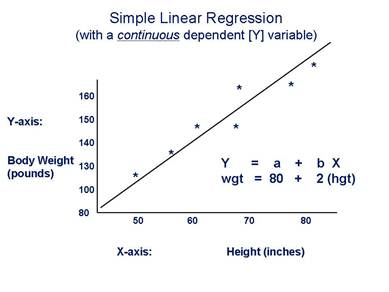
\includegraphics[center]{simpleLinearRegression}
	\caption[Confusion Matrix]
	{Simple Linear Regression}
	\label{fig:simpleLinearRegression}
\end{figure}

We can see from above the $y$ in this example is weight (wgt) and $b_0 + b_1x$ is $80 + 2*Height(hgt)$. This is a very basic example but demonstrates how this can be leveraged for more complex feature sets. Predicting arrears is a dichotomous problem meaning the outcome of the experiment can only have two possible values. 

\subsection{Logistic Regression} \label{LogReg}
\textit{Logistic Regression} \cite[See:][]{hosmer_applied_2000} within the credit scoring industry is one of the most used algorithms \citep{hand_evaluating_2010}. As seen above in Fig. \ref{fig:simpleLinearRegression} a simple regression model outputs a continuous response, in that example body weight. Credit scoring or predicting arrears is a problem where there can only be two possibly values default or not-default, to simplify this we will reduce this to a binary problem where the outcome will be 1 or 0 \citep{zou_modified_2004}. To transform the output of a regression model from $[-\infty, +\infty]$ to a probability between 0 and 1 a logistic transformation is applied. The logistic function can be used to take any value between $+\infty$ and $-\infty$ and output a value between $0$ and $1$. Fig. \ref{fig:logistic_function} below illustrates what a logistic function looks like.


\begin{figure}[H]
	\includegraphics[width=0.6\textwidth, center]{logistic_function}
	\caption[Standard Logistic Regression]
	{Standard Logistic Regression}
	\label{fig:logistic_function}
\end{figure}

The logistic function is defined in Equation \ref{eq:logitReg} as the following: 

\begin{equation} \label{eq:logitReg}
	\text{Logistic Model}  =  p  =  \frac{1}{1 + e^{-(b_0 + b_1x)}}
\end{equation}

As discussed already linear regression is an unsuitable classifier for making dichotomous predictions as linear regression produces predictions for a range beyond 0 to 1. Logistic regression also produces a curved line that is bounded by values between 0 and 1. Fig. \ref{fig:LogRegVsLineReg}

\begin{figure}[H]
	\includegraphics[width=0.6\textwidth, center]{LogRegVsLineReg}
	\caption{Comparison between Linear and Logistic Regression Models}
	\label{fig:LogRegVsLineReg}
\end{figure}

in \ref{fig:LogRegVsLineReg} the constant, $b_0$ dictates the position of the curve which can be moved left and right depending on its value, $b_1$ will be the slope of the curve. 

The logistic regression model can be extended to include any number of interval and nominal variables which is illustrated in Equation \ref{eq:logitRegExtended}

\begin{equation} \label{eq:logitRegExtended}
	p  =  \frac{1}{1 + e^{-(b_0 + b_1x_1 + b_2x_2 +\cdot\cdot\cdot+ b_px_p )}}
\end{equation}

Logistic Regression can also be used in cases where there are more than two outcome groups. For example it could be used in predicting what stage a customer is in the customer lifecycle e.g. Awareness, Interest/Consideration, Evaluation/Purchase, this is referred to \textit{multinomial logistic regression}


One of the main major attractions of logistic regressions it allows you to use discrete, continuous features or a combination of both \citep{lee_application_2005}.

\subsection{K-Nearest Neighbours} \label{kNN}
The \textit{k-nearest neighbour} or {k-NN} for short, is an algorithm that classifies observations based on the how its nearest neighbours are classified. It can be known as the nearest neighbour but in the majority of cases it is useful to use more than one neighbour \citep{henley_k-nearest-neighbour_1996}. The intuition behind this algorithm is that instances which are close by each other will more likely be classified the same way \citep{cover_nearest_1967}. We can see in Fig. \ref{fig:KNN_Example}\\ %added space for small gap in picture 


\begin{figure}[H]
	\includegraphics[width=0.6\textwidth, center]{KNN_Example}
	\caption{Example k-NN, contrasting results for \textit{k}=3 and \textit{k}=5 }
	\label{fig:KNN_Example}
\end{figure}

that results of the algorithm can vary with the choice of \textit{k}. It should also be noted that when applying this algorithm to binary experiment it is good practice to only choose odd values of \textit{k}, this will eliminate the risk of ties from the decision process \citep{keller_fuzzy_1985} 

While adopting the k-NN algorithm you can choose which method and validate what the best distance measure to decide what are your nearest neighbours. There are some common distance measures for continuous features only, Equation \ref{eq:Minkowski} is the \textit{minkowski distance} is one of the most common, where \textit{p=1} this becomes the Equation \ref{eq:Manhatten} the \textit{manhatten distance} and where \textit{p=2} this becomes the Equation \ref{eq:Euclidean} the \textit{euclidean distance}

\begin{equation} \label{eq:Minkowski}
	\text{Minkowski Distance}   = \Big(\sum_{i=1}^k (\abs{x_i-y_i})^p\Big)^\frac{1}{p}
\end{equation}

\begin{equation} \label{eq:Manhatten}
	\text{Manhatten Distance}   = \sum_{i=1}^k \abs{x_i-y_i}
\end{equation}

\begin{equation} \label{eq:Euclidean}
	\text{Euclidean Distance}   = \sqrt{\sum_{i=1}^k (x_i-y_i)^2}
\end{equation}

The results from k-NN will vary depending on your choice of distance measurement, but there more distance metrics for continuous features such as \textit{Correlation Similarity}, \textit{Cosine Similarity} \citep{sarwar_item-based_2001}

Analysis can be completed to evaluate what the optimal value for \textit{k} is based on inspecting the results and creating benchmarks. Anecdotally the larger the value of \textit{k} the more precise the algorithm can be but as with most things in machine learning there are no guarantees. You can leverage methods such as cross validation discussed in Section \ref{subsec:k_fold} and utilised in Chapter \ref{Chapter4} to evaluate what the good choice of \textit{k} would be.

\subsection{Decision Trees} \label{decTrees}
The \textit{decision tree} algorithm classifies observations into classes in the form of tree like structure, hence the name. The algorithm seeks to partition the dataset into smaller subsets, using the relationship between the feature set and target variable to do so. Fig. \ref{fig:decisionTree}

\begin{figure}[H]
	\includegraphics[width=1\textwidth, center]{decisionTree}
	\caption{Simple Decision Tree for Yes, No Prediction \\ \cite[Source:][]{quinlan_induction_1986}}
	\label{fig:decisionTree}
\end{figure}

The output of the algorithm splits the data into smaller subsets of data, which output is a tree with root, internal and leaf nodes. As can be seen in Fig. \ref{fig:decisionTreeExplained}, the root node in this example \textit{Outlook} is the first node in the tree which means it is the most predictive feature. 

\begin{figure}[H]
	\includegraphics[width=.6\textwidth, center]{decisionTreeExplained}
	\caption{Decision Tree with Nodes and Leafs labelled}
	\label{fig:decisionTreeExplained}
\end{figure}

The \textit{root node} will have have two or more branches in this case three \textit{Rainy, Overcast} and \textit{Sunny}. Below these branches you have \textit{internal or split node} \textit{Windy} or \textit{Humidity} which output more branches. The bottom nodes of each decision or branch is the prediction or classification, this is called the \textit{leaf node}. In this example the leaf node decision will be whether or not it will rain represented by Yes/No in Fig. \ref{fig:decisionTreeExplained}

The algorithm that builds decision trees is called the \textit{iterative dichotomiser 3} more commonly known as ID3 by \cite{quinlan_induction_1986}. The algorithm applies a top down approach to choosing its root and internal nodes. The algorithm only evaluates one step ahead from where it is in the decision process at any time and does not allow for any backtracking. This decision making process is known as a greedy approach as it just makes the optimal solution at that stage of the process. Thus because of these limitations the optimal solution is not guaranteed taking this approach \citep{friedman_lazy_1996}.

The ID3 algorithm works by calculating the \textit{entropy} and \textit{information gain} at each step or decision node, where you use the feature with the smallest entropy or feature that maximises information gain.

Entropy $H(S)$ seen in Equation \ref{eq:entropy} measures how much uncertainty there is in the data \citep{shannon_mathematical_2001}

\begin{equation} \label{eq:entropy}
	H(S) = - \sum_{x \in X} p(x) \log_{2} p(x)
\end{equation}
Where:
\begin{itemize}[label=]
	\item $S$: The current dataset entropy is being calculated for, this will change each time entropy is being calculated
	\item $X$: The set of classes in $S$
	\item $p(x)$: Proportion of observation in class $x$ compared to total number in set $S$
\end{itemize}
If $H(S) = 0$ then the observations in $S$ are all of the same class. Entropy is calculated for each feature, the feature with the smallest entropy is used to split at that step.

Information gain is used to measure the decrease in entropy after the dataset is split on a feature. The equation for the information is 

\begin{equation} \label{eq:infoGain}
	IG = H(S) -  H(T)
\end{equation}
Where:
\begin{itemize}[label=]
	\item $H(S)$ is the the entropy of S
	\item $H(T)$ is the entropy of subset T based on splitting data on some feature
\end{itemize}

Information gain is calculated and the feature with the highest gain is chosen to split the dataset. The algorithm then runs recursively until all the data is classified and predictions have been made. 

Multiple decision trees may output the same results. This can be seen in Fig. \ref{fig:simpleComplex} where two different decision trees classify the dataset correctly. \cite{quinlan_induction_1986} suggests that that in scenarios like this the simpler decision tree would be chosen Fig. \ref{fig:simple}

\begin{figure}[H]
	\centering
	\begin{subfigure}[b]{0.45\textwidth}
		\captionsetup{font=scriptsize}
		\includegraphics[width=\textwidth, height=5cm]{decisionTreeSimple}
		\caption{Simple Decision Tree}\label{fig:decisionTreeSimple}
		\label{fig:simple}
	\end{subfigure} ~\quad
	\begin{subfigure}[b]{0.45\textwidth}
		\captionsetup{font=scriptsize}
		\includegraphics[width=\textwidth,height=5cm]{decisionTreeComplex}
		\caption{Complex Decision Tree}\label{fig:decisionTreeComplex}
		\label{fig:complex}
	\end{subfigure}
	\caption{Simple and Complex Decision Tree Comparison\\\cite[Source:][]{quinlan_induction_1986}}
	\label{fig:simpleComplex}
\end{figure}

This is done because the simpler the rules of the tree the more likely the tree is to generalise well on unseen data. In other words if the tree is too complex it is more than likely over-fitting the training dataset. There is also a computational cost to classifying complex trees. 

There are also other issues to be aware of when building a classifier using a decision tree. Information gain can be biased to features that have a large number of values. These features will result in a root node that produces a very broad or wide tree that classifies the training data well or perfectly but performs very poorly in unseen cases. One scenario where this could happen would be if you used the unique identifier of each record in as a training input, this model would perform very well in training but would not perform well on unseen data. There are methods to mitigate the the risk of over-fitting against these features \textit{gain ratio}, \textit{symmetric uncertainty} and the \textit{gini index}. \cite{quinlan_induction_1986} noted that using these methods for node decision often found favourable results compared with information gain. It should be noted also that these metrics can be using in the feature selection process where not related to building decision trees


\subsection{Artificial Neural Networks} \label{neuralNets}
The \textit{artificial neural network} (ANN) is learning algorithm that is based on an understanding of how neural networks, such as our brain learns. Motivation to study how ANN comes from the success of how the human brain was faster than the worlds fastest computers at certain applications such as object recognition, speech recognition and general perception \citep{haykin_neural_1998}.

As a human grows their brain develops, learns and creates a set rules based on the experiences it has had. These rules and experiences are stored in approximately 100 billion neurons or nerve cell in the brain. These neurons are connected in a network and use this as a method of communication sending electrical and chemical signals back and forth between neurons. On their own each neuron is not very useful but combined and with communication has allowed humans to learn and grow so successfully. 

An ANN seeks to replicate the neural network of the human brain, albeit on a much smaller scale. It does this by taking advantage of powerful computers which carry out a lot of simple tasks very quickly. ANN have proven their value from their ability to map out any non-linear function \citep{white_learning_1989} and their prowess in applications such as pattern and speech recognition and forecasting \citep{kaastra_forecasting_1995}.

Fig. \ref{fig:annFotwardFeeding} shows a common layout of an ANN. Like in the brain the ANN is comprised of processing neurons usually known as nodes which are organised into three layers, input, hidden and output. Between layers nodes are connected and as seen in Fig. \ref{fig:annFotwardFeeding} each connection may carry a different weight.

\begin{figure}[H]
	\includegraphics[width=.6\textwidth, center]{annFotwardFeeding}
	\caption{Three-layered feed-forward artificial neural network configuration \\
				\cite[Source:][]{raju_development_2011}
			}
	\label{fig:annFotwardFeeding}
\end{figure}

Data comes in through the input layers nodes and is fed through the network, from the input to the hidden and then onto the output layer. In the hidden layer each node calculates a sum based on the input node and the weight of the connection, these hidden nodes then pass on values to the nodes in the outer layer where another calculation which converts the value to a value between 0 and 1 by passing it through the sigmoid function seen in Fig. \ref{fig:logistic_function}. Throughout the training process the connection weights are changed and tested against in order for the ANN to learn and improve its predictions \citep{haykin_neural_1998}

Although ANN have become increasingly popular in recent years due to improvements in the algorithms, the the increase in computer power and success in application such as object and speech recognition,  some are still sceptical because of the "black box" nature of their results, where users do not know what the internal workings of the algorithm are  \citep{kaastra_forecasting_1995}. 



\subsection{Support Vector Machines} \label{SVM}
A Support Vector Machines (SVMs) learning was developed first by \cite{vapnik_nature_1995}. The algorithm performs classifications via a hyperplane in a higher dimensional feature space that maximises the margin or distance separating the two classes. It can be seen in Fig. \ref{fig:svmExample} that the two class are linearly separable using the hyperplane in the higher dimensional feature space. 

\begin{figure}[H]
	\includegraphics[width=.5\textwidth, center]{svmExample}
	\caption{Optimal separating hyperplane in SVMs of feature space \\
		\cite[Source:][]{li_adaptive_2011}
	}
	\label{fig:svmExample}
\end{figure}

SVM handles situations non-linear data by using kernel function (non linear) to transform the data into a higher dimensional feature space. This allows it to become linearly separable via a hyperplane, this is known as the \textit{kernel trick}. It can illustrated in Fig. \ref{fig:svm_nonLinearlySeperable} by transforming non linearly seperable data into a higher dimensional feature space where it can be linearly separated using a hyperplane. This is ability is what differentiates SVM from logistic regression.

\begin{figure}[H]
	\includegraphics[width=.5\textwidth, center]{svm_nonLinearlySeperable}
	\caption{SVM classifying non-linearly classes \\
		\cite[Source:][]{burges_tutorial_1998}
	}
	\label{fig:svm_nonLinearlySeperable}
\end{figure}

It has been documented across a range of domains where SVMs are performing well such as credit risk evaluation \cite{van_gestel_credit_2009} and text categorisation, cancer diagnosis and pattern recognition \citep{shin_application_2005}

\subsection{Ensemble models \& Boosting} \label{boosting}
\begin{comment}
In 1907, statistician Sir Francis Galton attended a fair in which there was a competition to judge the weight of an Ox. Upon reviewing the 787 predictions made by the competing public, he observed that while there was a 
\end{comment}


%----------------------------------------------------------------------------------------
%	SECTION 6
%----------------------------------------------------------------------------------------
\section{Model Building and Training}
sasasas
\subsection{Class Imbalance Problem}
One of the biggest assumptions that needs to be understood when using classification algorithms is that most assume there is a balanced distribution of the target class \citep{japkowicz_class_2000}. Target class imbalance is described by  \citep{chawla_smote:_2002} where the number of number of records in each class are not relatively equal. In a balanced dataset ratio between the a binary target class would be close to 50/50. The issue with this imbalance arises where algorithms assume there is a balance between the classes, and they attempt to maximise the accuracy by predicting the most common class \citep{drummond_severe_2005}. The algorithms attempt to minimise the classification errors, but do not accounts for the incorrectly classifying cases \citep{seiffert_improving_2009}. While these classification overall might be very accurate they are not very useful in real world problems, this is because in the majority of cases the algorithm will focus on the majority class, because of how heavily it is weighted in the training dataset ignoring the minority class. This is major problem because in the majority of cases you will trying to predict the minority class, in this thesis customers going into default is the minority e.g. there are more customers that do not default at the end of the outcome window than customers that do defaulters.

The study of class imbalance has started to receive more and more attention in relation to data mining and machine learning in recent times. \cite{weiss_mining_2004} discusses what the role and issue that rare class instances can play in data mining. \cite{weiss_mining_2004} makes the distinction that there are two types of class imbalance which depend on the type of rarity in the data, these are called \textit{absolute rarity} and \textit{relative rarity} which are discussed next.

The major issue with rarity is there is a simply a lack of data in real world problems. Absolute rarity occurs when the number of instances related to the rare class is very small in an absolute sense. Lack of data means it is difficult to identify what leads to a rare class. Fig. \ref{fig:absoluteRarity} illustrates how absolute rarity can become an issue.

\begin{figure}[H]
	\includegraphics[width=0.6\textwidth,center]{absoluteRarity}
	\caption{
		Impact of Absolute Rarity in Data Mining \\ \cite[Source:][]{weiss_mining_2004}
	}
	\label{fig:absoluteRarity}
\end{figure}

It can be seen on the left side of Fig. \ref{fig:absoluteRarity} that there is only one rare/positive example, compared to the right where there is more data this more rare cases. It can be observed that the decision boundary on the right side for when there is more data is much more accurate than on the left side when there is just one observed rare class. This is a simple illustration that having more data should allow you to make better predictions. Relative rarity is where classes are not rare in an absolute sense but are rare relative to other objects. A supermarket example can illustrate this better, imagine you want to identify the relationship between two items, but these items are rarely purchased as whole, so even if they happen to be purchased together the relationship may be difficult to identify.

As mentioned previously, very often in the real world problems imbalance exists in the dataset, thus there has been researched completed that have identified methods of mitigating against this risk. \citep{chawla_editorial:_2004} proposes solutions fine tuning the algorithm and manipulating the data. 

\subsubsection{Manipulating the data}

A method of manipulating the data is to resample to data with the aim of balancing the distribution of the target class. Solutions proposed,

\begin{itemize}
	\item Random undersampling the majority class
	\item Random oversampling the minority Class
	\item Synthetic of the minority Class 
\end{itemize}

A very common method used is to randomly oversample the minority class in your training set, one of the biggest issues with this is that you are increasing your chances of over-fitting the algorithm the training model as it been training on multiple copies of the same data which are not adding any new information. However over-fitting can be issue with this approach as the algorithm becomes biased and skewed on the training data, thus ends up performing poorly on the validation and test data \cite[see][]{hawkins_problem_2004}

Random undersampling of the minority class is where random samples of the training dataset that are part of the majority class are removed. This means number of minority classes remains unchanged but the majority class is reduced, thus the overall class balance becomes more even. The issue that arises from undersampling is that there is possibility that you removes the important information from the training dataset that is used for predicting that class. It should be noted \cite{kennedy_credit_2013}, that undersampling the majority class is not a useful solution for the issue of absolute rarity.

Synthetic sampling  is alternative method to randomly oversampling the minority class. New data items are added to the training set but unlike oversampling which adds duplicate records the records added are dummy or made up in a way to look similar and taking characteristics of the already existing records, thus they are not duplicates but synthetic. One method for creating synthetic data was proposed by \citep{chawla_smote:_2002} where data was generated by creating data items using K-NN where the item would sit between minority classes. 

\begin{figure}[H]
	\centering
	\begin{subfigure}[b]{0.32\textwidth}
		\captionsetup{font=scriptsize}
		\includegraphics[width=\textwidth]{SMOTE_Before}\caption{}
		\label{fig:SMOTE_Before}
	\end{subfigure}  ~\quad
	\begin{subfigure}[b]{0.32\textwidth}
		\captionsetup{font=scriptsize}
		\includegraphics[width=\textwidth]{SMOTE_After}
		\caption{}
		\label{fig:SMOTE_After}
	\end{subfigure}
	\caption{Fig. \ref{fig:SMOTE_Before}: Example of the K-NN for $x_i$ using $k = 6$. \ref{fig:SMOTE_After}: Data created using SMOTE based on the euclidean distance.\\
		\cite[Source:][]{he_learning_2009}}
	\label{fig:smoteExample}
\end{figure}

Above in Fig. \ref{fig:smoteExample} it is illustrated how synthetic data using the SMOTE methodology can be generated. For the purposes of this thesis this will not be discussed further.

\subsubsection{Fine tuning the algorithm}
There are ways to also cater for the target class imbalance of the dataset by fine tuning the algorithm. One method which is illustrated in Chapter \ref{Chapter4} of this thesis is to adjust the cut-off or threshold parameter value for the model, \cite{provost_machine_2000} warns that it would \textit{``critical mistake"}. In Section \ref{modelPerformMeasure} model performance measures, it is  worth noting that \cite{chawla_editorial:_2004} suggests using evaluation measures such as accuracy which rely on a specific threshold could lead to misleading results when the target class is imbalanced, they instead recommend using ROC and AUC to get a more accurate predictions, this similar to industry standards in terms of handling the imbalance.

This section has detailed some of the concern that imbalance can cause when building predictive models, we have outlined some the solutions and methods to mitigate this by manipulating the data and fine tuning the classification algorithm.


\subsection{Feature Selection}
\subsubsection{Correlation-based Feature Selection}
\subsubsection{Information Gain}
\subsubsection{Coarse Classification/ Binning}



%----------------------------------------------------------------------------------------
%	SECTION 7
%----------------------------------------------------------------------------------------
\section{Model Validation Methods}
In machine learning historic data is used to build a model to make future predictions based on past information. Classification algorithms like the ones already discussed in this section need to validated and tested. This section details some methods and approaches to tackling this problem so the predictions from the model are useful which has been discussed extensively in \citep{refaeilzadeh_cross-validation_2009}

\subsubsection{Resubstitution Validation}
The \textit{resubstitution validation} method the model is trained using the full dataset available, and afterwards tested using the same dataset. The results of this test will most likely be positive, but there os a danger that the model will perform poorly on unseen data because it because it is over-biased and over-fits the training data

\subsubsection{Holdout Validation}
The \textit{holdout validation} method is used to avoid the over-fitting issue discussed in the resubstitution method. The idea is to split the data into partitions, one for training and one for testing. The algorithm is only trained on the test data, this allows for the model to generalise much better on unseen data, overall producing a much better prediction model. This method has an issue however where one, not all the data is used for training, and two the results can be dependent on the how and what data are used for training and testing. Examples where this could become an issue is important information in the data for training is lost in the test partition, or the instances chosen for test may be too easy or too difficult to classify, this may cause your results to be skewed and making your predictions bias to that testing partition.

\begin{figure}[H]
	\includegraphics[width=0.6\textwidth,center]{holdout}
	\caption{Example of Holdout Validation Data Split}
	\label{fig:holdout}
\end{figure}

Fig. \ref{fig:holdout} illustrates how the complete dataset is partitioned into a training and test sets. To address the biasses is Holdout you could re-run multiple tests and average the results, or more commonly you could look at using \textit{k-fold cross-validation} discussed in the next subsection.

\subsubsection{K-Fold Cross Validation}\label{subsec:k_fold}
The \textit{k-fold cross validation} can be used to deal with the bias issues discussed above. The first step of this method is to split the data into $k$ equally sized partitions called folds. A model is then trained using $k$ iterations, where for each iteration a different fold of data is used for testing and training the model. This can be illustrated well below in Fig. \ref{fig:5-fold-cv} where there are 5-folds, and for each iteration you can see different fold is being used for testing.  

\begin{figure}[H]
	\includegraphics[width=0.7\textwidth,center]{5-fold-cv}
	\caption{5-Fold Cross Validation}
	\label{fig:5-fold-cv}
\end{figure}

It is important and usually common practice that each fold is representative of the the whole dataset, for each example that the target class ratio split is the same for each fold as for the entire dataset. 

\subsubsection{Leave-One-Out Cross-Validation}
The \textit{leave-one-out cross-validation} (LOOCV) method is a specialised version of $k$-fold cross-validation, where $k$ is equal to the number of observations in the dataset. In layman's term this means all the data bar one observation is utilized training the model, and testing is done on one observation. This is completed for each observation in the dataset. Although it is worth noting that accuracy estimate gathered using this method produces unbiased results, it also high variance which can lead to misleading results \citep{refaeilzadeh_cross-validation_2009}.
 

\subsubsection{Repeated K-Fold Cross Validation}
The \textit{repeated k-fold cross validation} method is another specialised version of $k$-fold cross-validation. In an attempt to improve the performance of the model using this method $k$-fold cross-validation is rerun multiples times. Each time it is rerun the data is shuffled so data will appear in different folds for each repeat run. 

\subsubsection{Summary}

Holdout and cross validation methods are both used extensively for evaluating how measuring the performance of the models. In the majority of cases if there is a large enough dataset you might choose to just use holdout method, but in some situations of you may want to use cross validation.

There are considerations that need to be thought about before using either, hold-out is simple can be implemented easily and quickly and can be rerun multiple times to get a more unbiased result. K-fold is again theoretically simple but may not be a simple to implement as the code may be tedious and time consuming where the gains may not be worth the investment in industry. 

\citep{kohavi_study_1995} and \citep{salzberg_comparing_1997} both performed research on approaches to choosing the correct validation method. \cite{kohavi_study_1995} analysed many cross validation methods, regular, leave-one-out, stratified. They came to the conclusion that 10-fold cross-validation produced the most accurate and unbiased results. \cite{salzberg_comparing_1997} also studies the issues of comparing model performance and proposes a solution that combines k-fold cross validation combined appropriate hypothesis tests opposed to evaluating the average accuracy.   



%----------------------------------------------------------------------------------------
%	SECTION 8
%----------------------------------------------------------------------------------------
\section{Model Performance Measures}\label{modelPerformMeasure}

This section details some of the metrics that can be used to assess the accuracy of a classifier. The result of the classification algorithm maps the modelled data into a category, in this thesis it a binary classifier that is output: 1 is output for identifying customers who will default (bad) or 0 is output for customers who will be not-default (good). The majority of classification algorithms will produce a ranked numeric value which can be converted to a binary representation by some threshold or cut-off decision driven from  the business objective that is trying to be optimised. This section will begin with a confusion matrix, details how this is leveraged to build other performance measures and details how charts and metrics can be leveraged together to decide on the performance measure to maximise the intended objective.

\url{http://www.saedsayad.com/model_evaluation_c.htm}

\subsubsection{Confusion Matrix}

The results that made by the classification algorithm can be represented by a contingency table known as a confusion matrix. In this thesis the classification algorithm will output a binary classification, so the confusion matrix will be made from a $2 \times 2$ matrix that has two classes, known as the \textit{positive} and \textit{negative} class. For this thesis, the positive class will be the customers that default and negative class will be the customers that do not default. It will illustrate what proportion of correct and incorrect predictions were made with respect to the target.The confusion matrix can be broken down into the following categories for this thesis:

\begin{itemize}
	\item \textit{true positive} (TP), cases that are predicted to default, and are {\color{green}{correctly}} classified as \textit{positive}
	\item \textit{false positive} (FP), cases that are predicted to default, and are {\color{red}{incorrectly}} classified as \textit{positive}, also known as \textit{Type I error}.
	\item \textit{false negative} (FN), cases that are predicted to not-default, and are {\color{red}{incorrectly}} classified as \textit{negative}, also known as \textit{Type II error}.
	\item  \textit{true negative} (TN), cases that are predicted to not default, and are {\color{green}{correctly}} classified \textit{negative}
	
\end{itemize}

Fig \ref{fig:ConfusionMatrix} illustrates how information from a confusion matrix can be presented and read.

\begin{figure}[H]
	\includegraphics[width=0.8\textwidth,center]{Confusion_Matrix}
	\caption[Confusion Matrix]
	{Confusion Matrix}
	\label{fig:ConfusionMatrix}
\end{figure}

Using the numbers outputted from the confusion matrix, model evaluation measures can calculated and evaluated for the required objective, measures such as \textit{accuracy} (Equation \ref{eq:Accuracy}) which measures proportion of the number of predictions that were correct, the \textit{misclassification rate} (Equation \ref{eq:Misclassification Rate}) what proportion of predictions were wrong, the \textit{sensitivity} (Equation \ref{eq:Sensitivity}), otherwise known as \textit{recall} or the \textit{true positive rate} (TPR), measures the proportion of the positive instances that are correctly identified i.e. proportion default cases that have been predicted correctly. \textit{Specificity} (Equation \ref{eq:Specificity}) measures the proportion of negative cases that are predicted correctly i.e. proportion of non-default cases that have been predicted correctly, \textit{precision} (Equation \ref{eq:precision}) measures when the classifier predict positive outcomes what proportion are correct, \textit{negative predictive value} (NPV) (Equation \ref{eq:npv}) measures the proportion of negative predictions that were correct i.e. if the classifier predicted the outcome would be non-default what proportion were correct. One measure that can be very useful when the where there is class imbalance is \textit{balance accuracy} (Equation \ref{eq:Balanaced Accuracy}), \citep{brodersen_balanced_2010} discusses how using this negates the impact of bias or skewness from the more frequent class

\begin{equation} \label{eq:Sensitivity}
\text{Sensitivity} = \text{Recall} = \frac{TP}{TP + FN}
\end{equation}

\begin{equation} \label{eq:Specificity}
\text{Specificity} = \frac{TN}{FP + TN}
\end{equation}

\begin{equation} \label{eq:precision}
\text{Precision} = \frac{TP}{TP + FP}
\end{equation}

\begin{equation} \label{eq:npv}
\text{Negative Predictive Value} = \frac{TN}{TN + FN}
\end{equation}

\begin{equation} \label{eq:Accuracy}
\text{Accuracy} = \frac{TP + TN}{TP + FP + FN + TN}
\end{equation}

\begin{equation} \label{eq:Balanaced Accuracy}
\text{Average Accuracy} = \text{Balanaced Accuracy} = \frac{Sensitivity + Specificity}{2}
\end{equation}

\begin{equation} \label{eq:Misclassification Rate}
\text{Misclassification Rate} =  \frac{FP + FN}{TP + FP + FN + TN} = 1 - \text{Accuracy}
\end{equation}

\begin{figure}[H]
	\includegraphics[width=0.8\textwidth,center]{Confusion_Matrix_Example}
	\caption[Confusion Matrix Example]
	{Confusion Matrix Example}
	\label{fig:ConfusionMatrixExample}
\end{figure}

Fig. \ref{fig:ConfusionMatrixExample} illustrates how the TP, FP, FN, TN can be used to create performance metrics for classification algorithm. As discussed already confusion matrix based performance measures are built on the threshold that is selected for converting the predicted numeric score into a binary outcome. Anecdotally you might believe that the cut-off or threshold of 0.50 is acceptable but this rule may not always especially if there is an imbalance between the positive and negative class in the dataset. The cut-off should should ideally be based on you business objective where you look to minimise, maximise and analyse the trade off as you alter the cut-off. 

The confusion matrix is not the only way to evaluate the performance of the classification algorithm and is not always advocated in the literature or by industry. In studies completed by \citep{lessmann_benchmarking_2008} choose not to select a classification cut-off arguing that studies comparing the same dataset and classifier could come to the different conclusions.

As mentioned in this section the confusion matrix measures the performance of classifier at a specific threshold, this can be leveraged to create graphical representations of the overall fitness of the model at any threshold. One such method that will be discussed in the next section is the \textit{receiver operating characteristic} (ROC). 


Confusion Matrix is used to evaluating a model where you have divided the output into distinct or discrete categories. A confusion matrix can be reconstructed for any point on the ROC curve. ROC is also is directly related to two other performance methods \textit{area under the curve} and \textit{gini} which will also be discussed.  

\subsubsection{ROC Chart, AUC and Gini Coefficient}
%\url{https://staesthetic.wordpress.com/2014/04/14/gini-roc-auc-and-accuracy/}
The ROC chart is used to evaluate and illustrate how well the evaluate the model fit, this can be a quick test to see if the model generalises well from the test data, to validation and test data. Fig. \ref{fig:ROC} illustrates on the \textit{x-axis} the false positive rate, and on the \textit{y-axis} the true positive rate is represented. As mentioned previously the points on the ROC chart are generated from confusion matrix built from many cut-off or threshold value between $\theta \in [0,1]$. Fig. \ref{fig:ROC} conceptually illustrates how the ROC chart is generated for varying thresholds. 

\begin{figure}[H]
	\includegraphics[width=0.8\textwidth,center]{ROC}
	\caption[ROC]
	{ROC Chart Example with thresholds 0.65 \& 0.50}
	\label{fig:ROC}
\end{figure}

Fig. \ref{fig:ROC} also illustrate how point (0,1) represents \textit{perfect classification}, that is the classifier correctly predicts all outcomes. 

The ROC chart is basically a combination of confusion matrices over many cut-off values of a classifier. As you can see above finite number of observations in the dataset dictates the number of thresholds that can be used to generate a ROC chart.

To compare ROC chart results of different classifiers the \textit{area under the ROC curve} (AUC) \citep{bradley_use_1997} \& \citep{hanley_meaning_1982}. In Fig. \ref{fig:ROC} the area under the blue ROC line represents the AUC, which is intuitively the area under the curve. In the case of perfect classification this value will be 1, for a random classifier the AUC would be 0.5. 

It is worth noting that AUC does not give total probability of the classifier, and also its usefulness when combined with the ROC to evaluate your classifier across training, validation and test datasets. For example if the ROC curve shifts significantly or is not similar from training to validation/test it suggests that there is possible over-fitting and the model does not generalise well. Also it is worth looking out for a drastic change in the AUC from training to validation/test another sign the classifier does not generalise well may not be useful for predictions. Because of this it is a very strong measure for classifier selection, ROC don't tend to cross over, therefore when comparing two classifiers the one which AUC is higher will be the better classifier independent of the threshold or cut-off.

It is illustrated in Fig. \ref{fig:matric_compare} how the performance measures for confusion matrices vary for different thresholds, but again to keep in mind that it there be just one measure for the AUC of the this ROC Chart.   

\begin{figure}[H]
	\centering
	\begin{subfigure}[b]{0.45\textwidth}
		\captionsetup{font=scriptsize}
		\includegraphics[width=\textwidth]{Confusion_Matrix_threshold_065}
		\caption{Threshold $=.65$}\label{fig:Threshold65}
	\end{subfigure} ~\quad
	\begin{subfigure}[b]{0.45\textwidth}
		\captionsetup{font=scriptsize}
		\includegraphics[width=\textwidth,height=2.025cm]{Confusion_Matrix_threshold_050}
		\caption{Threshold $=.50$}\label{fig:Threshold50}
	\end{subfigure}
	\caption{Confusion Matrix: Multiple Threshold Comparison}
	\label{fig:matric_compare}
\end{figure}

A metric that is commonly used for in \subjectname, industry credit scoring is the \textit{gini coefficient} this is discussed in \citep{hand_good_2005}, this is equates to twice the area in between the diagonal of a random classifier and the ROC curve. The equation for this can be seen below in Equation \ref{eq:gini}

\begin{equation} \label{eq:gini}
\text{Gini} = 2*\text{AUC} - 1
\end{equation}

Just like using a threshold there are limitations to using the AUC and Gini to measure classifier performance, although extremely useful for analysing the performance of wide range of thresholds but not as useful when trying to maximise the performance over a narrow range of thresholds. It cannot tell us the optimal threshold for classifier for  other statistical needs.

One statistic that is commonly used in credit scoring in \subjectname\, industry and in the literature is the \textit{kolmogorov-smirnov} (KS) statistic, this will be discussed in the next subsection.
	

\subsubsection{K-S Chart}\label{subsub:ks}
%\url{http://www.saedsayad.com/model_evaluation_c.htm}
The KS chart and more specifically the KS statistic is one value between 0 and 1. It can be used by measuring the performance of the classifier, by measuring the maximum distance between the cumulative positive and negative distributions of the predicted positive and negative class \citep{seliya_study_2009}. In other words K-S is a measure that illustrates the maximum seperation between the positive and negative distributions, this can illustrated more clearly in Fig. \ref{fig:ks}.

Fig. \ref{fig:ks} how the KS statistic and chart is generated, probabilities from the classifier are ordered, grouped and aggregated, but importantly they are separated by the positive and negative class, creating a distribution for each. These two distributions are then plotted separately, you can see in Fig. \ref{fig:ks} that the KS statistic is 47.4\%. This is calculated by taking maximum difference between the two distributions at each group. At group 400-500, if you were to classify all the score are positive below or in this group you would be identifying 81.7\% of the positive instance and only 34.3\% of the negative class, if this was a balanced dataset this could be a very valuable result and measure. 

\begin{figure}[H]
	\includegraphics[width=0.8\textwidth,center]{ks}
	\caption[Kolmogorov-Smirnov chart ]
	{Kolmogorov-Smirnov Table \& Chart }
	\label{fig:ks}
\end{figure}

There are extreme cases of the KS statistic that are worth noting, on is where the KS statistic is equal to 100, this means the scores for each distribution (positive/negative) are but into two separate groups, where one group would just have positive cases and the other just negative case. Alternatively if the model is not very useful and cannot tell the positives from the negatives, it will be like the model is selecting cases randomly and will return a KS statistic of 0.

We will see Chapter \ref{Chapter4} how this statistic can be utilised and leveraged to create a useful threshold value. 

\subsubsection{Gain \& Lift}
The \textit{gain} \& \textit{lift} measure the performance of the classifier. One example where these measure as charts are extremely useful is when communicating in industry with management, they are easy to explain and intuitive where the business can derive and understand value immediately. Fig. \ref{fig:GainLiftWorkflowCharts} below illustrates how the gain and lift charts are generated. 

\begin{figure}[H]
	\centering
	\begin{subfigure}[b]{0.90\textwidth}
		\captionsetup{font=scriptsize}
		\includegraphics[width=\textwidth,height=4cm]{gains_ratio_process}\caption{Process}\label{fig:gains_ratio_process}
	\end{subfigure} 
	\medskip
	\newline
	\begin{subfigure}[b]{0.45\textwidth}
		\captionsetup{font=scriptsize}
		\includegraphics[width=\textwidth]{gains}
		\caption{Gain Chart}\label{fig:gains}
	\end{subfigure} ~\quad
	\begin{subfigure}[b]{0.45\textwidth}
		\captionsetup{font=scriptsize}
		\includegraphics[width=\textwidth]{lift}
		\caption{Lift Chart}\label{fig:lift}
	\end{subfigure}
	\caption{Gain \& Lift Work-flow \& Charts}
	\label{fig:GainLiftWorkflowCharts}
\end{figure}

The charts above illustrate how much likely it is we receive positive responses using the classifier compared to use a random model. The population in the dataset are broken into deciles, which can be seen in \ref{fig:gains} \& \ref{fig:lift}. An example of how they can be used is if we were to evaluate the first 10\% of the population identified by the classifier it would outperform a random selection of customers that would turn out to positive by 3.6.

Essentially these charts are visual aids which can be leveraged for evaluating the performance of the classifier. 



%----------------------------------------------------------------------------------------
%	SECTION 9
%----------------------------------------------------------------------------------------
\section{Conclusion}\label{sotaConc}
This chapter has summarised the relevant literature available for ...
%----------------------------------------------------------------------------------------
%	SECTION 6
%----------------------------------------------------------------------------------------
